% This document has been prepared to help you approaching Latex as a formatting tool for your Travlendar+ deliverables. This document suggests you a possible style and format for your deliverables and contains information about basic formatting commands in Latex. A good guide to Latex is available here \href{https://tobi.oetiker.ch/lshort/lshort.pdf}{https://tobi.oetiker.ch/lshort/lshort.pdf}, but you can find many other good references on the web. 

% Writing in Latex means writing textual files having a \texttt{.tex} extension and exploiting the Latex markup commands for formatting purposes. Your files then need to be compiled using the Latex compiler. Similarly to programming languages, you can find many editors that help you writing and compiling your latex code. Here \href{https://beebom.com/best-latex-editors/}{https://beebom.com/best-latex-editors/} you have a short oviewview of some of them. Feel free to choose the one you like.  

% Include a subsection for each of the following items\footnote{By the way, what follows is the structure of an itemized list in Latex.}:
% \begin{itemize}
% \item
% Purpose: here we include the goals of the project
% \item
% Scope: here we include an analysis of the world and of the shared phenomena
% \item
% Definitions, Acronyms, Abbreviations
% \item
% Revision history
% \item
% Reference Documents 
% \item
% Document Structure
% \end{itemize}
% Below you see how to define the header for a subsection.

\subsection{Purpose}

\subsection{Scope}
... Here you see a subsubsection

\subsubsection{World Phenomena}
%what you write here is a comment that is not shown in the final text
In this section are introduced the environment related events that system can't perceive

\begin{figure}[H]
	\centering
    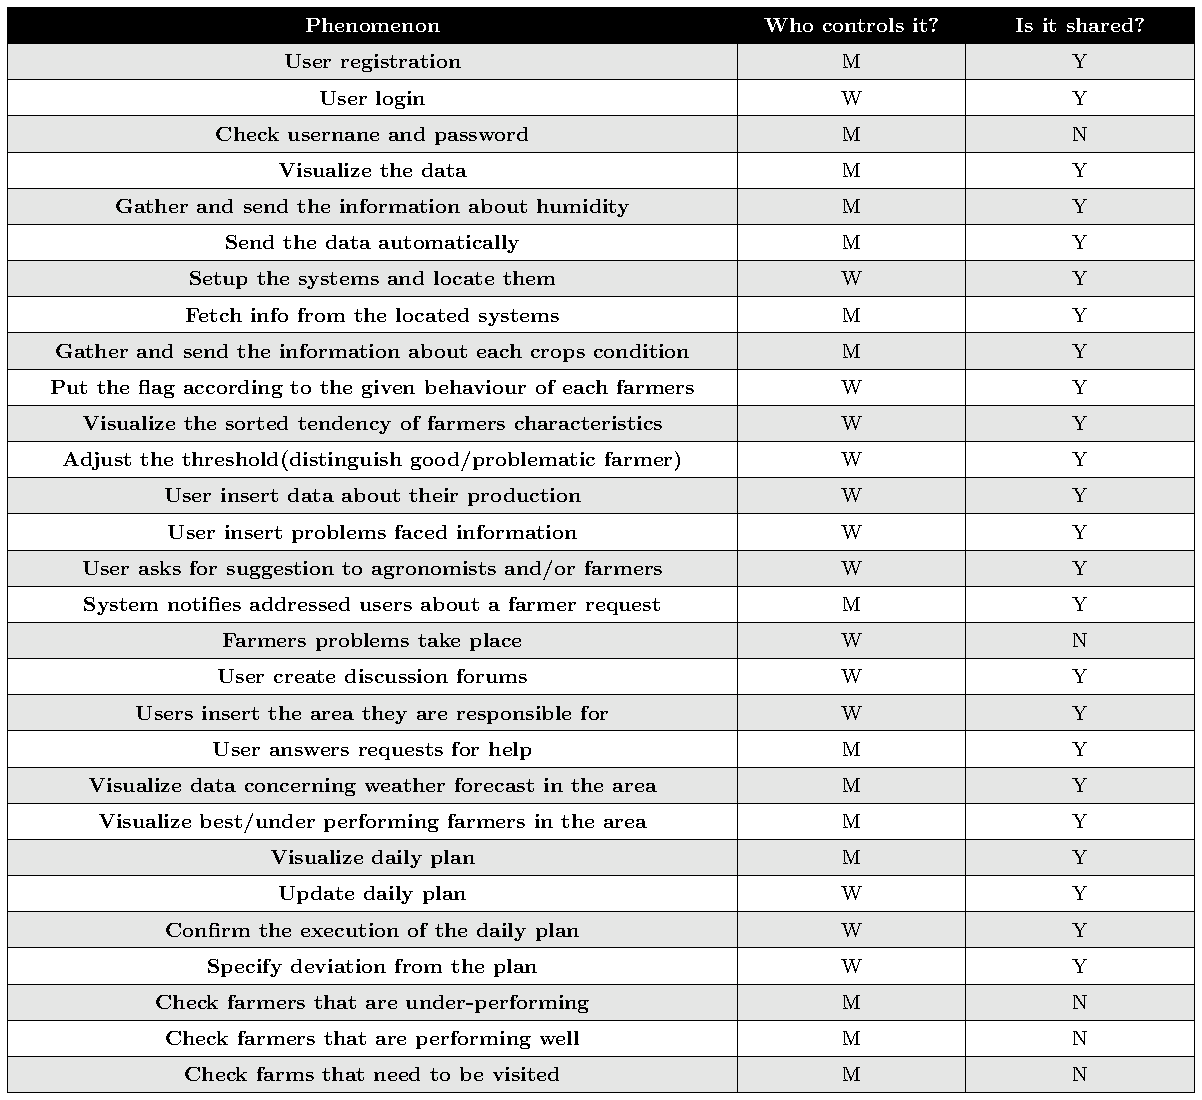
\includegraphics[page=1, width=\textwidth]{Tikz_stuff/Phenomena _table_external_project.pdf}
	\caption{\label{tab:phenomena}Phenomena table}
\end{figure}



\subsection{Goals}

\subsection{Definitions, Acronyms, Abbreviations}
% TODO Define verbs conventions of ISO/IEEE
% TODO Requirements should be ranked for importance or stability (from Hans Van Vliet book)
\subsection{Revision history}
		
\subsection{Reference Documents}
%% TODO
%% UNDP github repository and its sublinks, in particular Digital public goods standard website
% Hans Van Vliet software engineering book
% ISO/IEE document
% World/machine paper
% RASD assignment document
\subsection{Document structure}

